\documentclass[12pt,a4paper]{report}

% ============================================================================
% PACKAGES
% ============================================================================
\usepackage[utf8]{inputenc}
\usepackage[T1]{fontenc}
\usepackage{lmodern}
\usepackage[margin=1in]{geometry}
\usepackage{graphicx}
\usepackage{xcolor}
\usepackage{hyperref}
\usepackage{tikz}
\usepackage{longtable}
\usepackage{booktabs}
\usepackage{fancyhdr}
\usepackage{titlesec}
\usepackage{listings}
\usepackage{enumitem}

% TikZ Libraries
\usetikzlibrary{shapes.geometric, arrows.meta, positioning, fit, backgrounds, calc}

% ============================================================================
% COLORS
% ============================================================================
\definecolor{primaryblue}{RGB}{26, 54, 93}
\definecolor{secondaryblue}{RGB}{59, 130, 246}
\definecolor{accentgreen}{RGB}{34, 197, 94}
\definecolor{warningorange}{RGB}{249, 115, 22}
\definecolor{dangerred}{RGB}{239, 68, 68}
\definecolor{lightgray}{RGB}{243, 244, 246}
\definecolor{darkgray}{RGB}{75, 85, 99}
\definecolor{moneygold}{RGB}{234, 179, 8}

% ============================================================================
% HYPERREF SETUP
% ============================================================================
\hypersetup{
    colorlinks=true,
    linkcolor=primaryblue,
    urlcolor=secondaryblue,
    pdftitle={EduX - Fee Management Guide},
    pdfauthor={EduX Development Team},
}

% ============================================================================
% HEADER/FOOTER
% ============================================================================
\pagestyle{fancy}
\fancyhf{}
\fancyhead[L]{\textcolor{darkgray}{\small EduX School Management System}}
\fancyhead[R]{\textcolor{darkgray}{\small Fee Management Guide}}
\fancyfoot[C]{\textcolor{darkgray}{\thepage}}
\renewcommand{\headrulewidth}{0.4pt}

% ============================================================================
% TITLE FORMATTING
% ============================================================================
\titleformat{\chapter}[display]
  {\normalfont\huge\bfseries\color{primaryblue}}
  {\chaptertitlename\ \thechapter}{20pt}{\Huge}

\titleformat{\section}
  {\normalfont\Large\bfseries\color{primaryblue}}
  {\thesection}{1em}{}

\titleformat{\subsection}
  {\normalfont\large\bfseries\color{secondaryblue}}
  {\thesubsection}{1em}{}

% ============================================================================
% DOCUMENT
% ============================================================================
\begin{document}

% ----------------------------------------------------------------------------
% TITLE PAGE
% ----------------------------------------------------------------------------
\begin{titlepage}
    \centering
    \vspace*{2cm}
    
    {\Huge\bfseries\textcolor{primaryblue}{EduX}\par}
    \vspace{0.5cm}
    {\Large\textcolor{secondaryblue}{School Management System}\par}
    
    \vspace{2cm}
    
    
\begin{tikzpicture}
        \node[draw=primaryblue, line width=2pt, rounded corners=10pt, 
              minimum width=8cm, minimum height=3cm, fill=lightgray] 
              {\Huge\bfseries\textcolor{primaryblue}{Fee Management}};
    \end{tikzpicture}
    
    \vfill
    
    {\large\textcolor{darkgray}{Version 1.0}\par}
    {\large\textcolor{darkgray}{\today}\par}
\end{titlepage}

\tableofcontents
\newpage

% ============================================================================
% CHAPTER 1: OVERVIEW
% ============================================================================
\chapter{Fee Management Overview}

\section{Introduction}

The Fee Management module handles all financial aspects of student billing, from fee structure setup to payment collection and reporting.

\section{Fee System Components}

\begin{center}
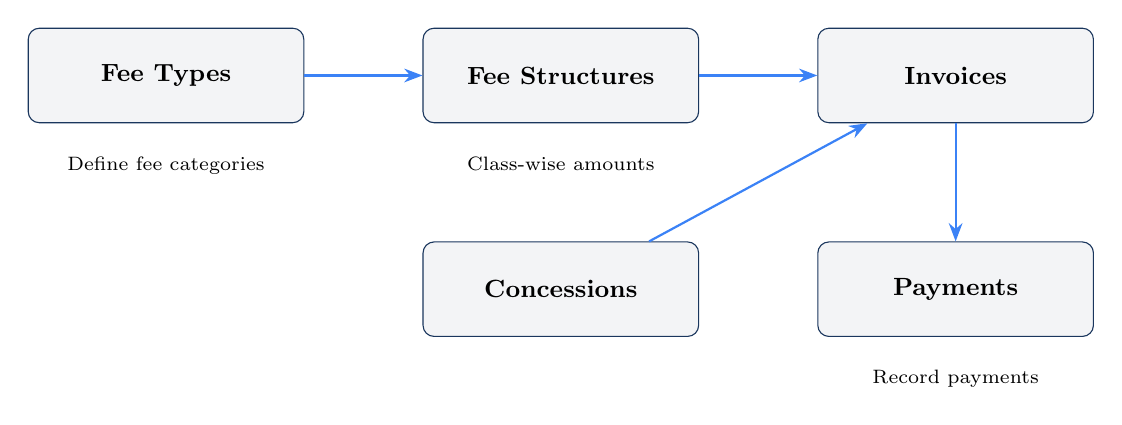
\begin{tikzpicture}[
    node distance=1.5cm,
    component/.style={draw=primaryblue, rounded corners, minimum width=3.5cm, 
                      minimum height=1.2cm, fill=lightgray, align=center, 
                      font=\small\bfseries},
    arrow/.style={-{Stealth}, thick, secondaryblue}
]
    \node[component] (types) {Fee Types};
    \node[component, right=of types] (structures) {Fee Structures};
    \node[component, right=of structures] (invoices) {Invoices};
    \node[component, below=of invoices] (payments) {Payments};
    \node[component, left=of payments] (concessions) {Concessions};
    
    \draw[arrow] (types) -- (structures);
    \draw[arrow] (structures) -- (invoices);
    \draw[arrow] (invoices) -- (payments);
    \draw[arrow] (concessions) -- (invoices);
    
    \node[below=0.3cm of types, font=\scriptsize, text width=3cm, align=center] 
        {Define fee categories};
    \node[below=0.3cm of structures, font=\scriptsize, text width=3cm, align=center] 
        {Class-wise amounts};
    \node[below=0.3cm of payments, font=\scriptsize, text width=3cm, align=center] 
        {Record payments};
\end{tikzpicture}
\end{center}

\section{Invoice Lifecycle}

\begin{center}
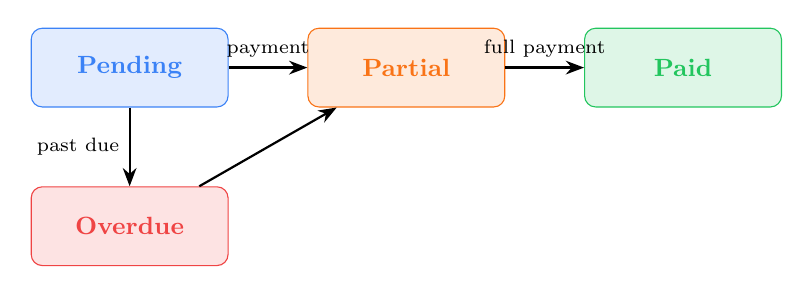
\begin{tikzpicture}[
    state/.style={draw=#1, rounded corners, minimum width=2.5cm, 
                  minimum height=1cm, fill=#1!15, font=\small\bfseries, text=#1}
]
    \node[state=secondaryblue] (pending) at (0,0) {Pending};
    \node[state=warningorange, right=1cm of pending] (partial) {Partial};
    \node[state=accentgreen, right=1cm of partial] (paid) {Paid};
    \node[state=dangerred, below=1cm of pending] (overdue) {Overdue};
    
    \draw[-{Stealth}, thick] (pending) -- node[above, font=\scriptsize] {payment} (partial);
    \draw[-{Stealth}, thick] (partial) -- node[above, font=\scriptsize] {full payment} (paid);
    \draw[-{Stealth}, thick] (pending) -- node[left, font=\scriptsize] {past due} (overdue);
    \draw[-{Stealth}, thick] (overdue) -- (partial);
\end{tikzpicture}
\end{center}

% ============================================================================
% CHAPTER 2: FEE TYPES
% ============================================================================
\chapter{Fee Types Configuration}

\section{Overview}

Fee Types define the categories of fees your school charges (e.g., Tuition, Transport, Lab Fee).

\section{Creating Fee Types}

Navigate to \texttt{Fees} $\rightarrow$ \texttt{Fee Types} $\rightarrow$ \texttt{Add}

\begin{longtable}{@{}p{4cm}p{3cm}p{6cm}@{}}
\toprule
\textbf{Field} & \textbf{Required} & \textbf{Description} \\
\midrule
\endhead
Name & Yes & Fee type name (e.g., ``Tuition Fee'') \\
Description & No & Detailed description \\
Is Monthly & Yes & Whether charged every month \\
Is Refundable & No & Can be refunded if student leaves \\
Account Code & No & For accounting integration \\
Display Order & No & Order in invoices \\
\bottomrule
\end{longtable}

\section{Common Fee Types}

\begin{center}
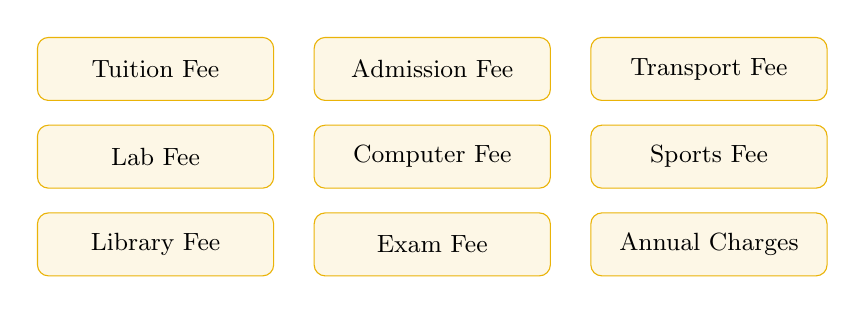
\begin{tikzpicture}[
    fee/.style={draw=moneygold, rounded corners, minimum width=3cm, 
                minimum height=0.8cm, fill=moneygold!10, font=\small}
]
    \matrix[row sep=0.3cm, column sep=0.5cm] {
        \node[fee] {Tuition Fee}; & \node[fee] {Admission Fee}; & 
        \node[fee] {Transport Fee}; \\
        \node[fee] {Lab Fee}; & \node[fee] {Computer Fee}; & 
        \node[fee] {Sports Fee}; \\
        \node[fee] {Library Fee}; & \node[fee] {Exam Fee}; & 
        \node[fee] {Annual Charges}; \\
    };
\end{tikzpicture}
\end{center}

% ============================================================================
% CHAPTER 3: FEE STRUCTURES
% ============================================================================
\chapter{Fee Structures}

\section{Overview}

Fee Structures define the actual amounts charged per class for each fee type.

\section{Creating Fee Structures}

Navigate to \texttt{Fees} $\rightarrow$ \texttt{Fee Structures}

\begin{enumerate}[leftmargin=*]
    \item Select \textbf{Class}
    \item Select \textbf{Fee Type}
    \item Enter \textbf{Amount}
    \item Set \textbf{Academic Year}
    \item Set \textbf{Effective From} date
    \item Save structure
\end{enumerate}

\section{Example Fee Structure}

\begin{center}
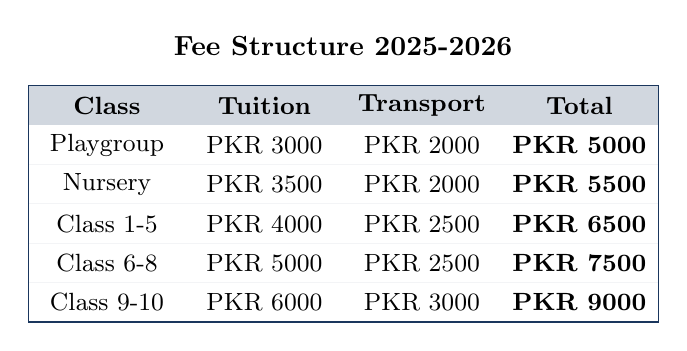
\begin{tikzpicture}
    % Table
    \node[font=\bfseries] at (4,3.5) {Fee Structure 2025-2026};
    
    % Headers
    \fill[primaryblue!20] (0,2.5) rectangle (8,3);
    \node[font=\small\bfseries] at (1,2.75) {Class};
    \node[font=\small\bfseries] at (3,2.75) {Tuition};
    \node[font=\small\bfseries] at (5,2.75) {Transport};
    \node[font=\small\bfseries] at (7,2.75) {Total};
    
    % Rows
    \foreach \y/\class/\tuition/\transport/\total in {
        2/Playgroup/3000/2000/5000,
        1.5/Nursery/3500/2000/5500,
        1/Class 1-5/4000/2500/6500,
        0.5/Class 6-8/5000/2500/7500,
        0/Class 9-10/6000/3000/9000
    } {
        \draw[lightgray] (0,\y) -- (8,\y);
        \node[font=\small] at (1,\y+0.25) {\class};
        \node[font=\small] at (3,\y+0.25) {PKR \tuition};
        \node[font=\small] at (5,\y+0.25) {PKR \transport};
        \node[font=\small\bfseries] at (7,\y+0.25) {PKR \total};
    }
    
    % Border
    \draw[primaryblue] (0,0) rectangle (8,3);
\end{tikzpicture}
\end{center}

% ============================================================================
% CHAPTER 4: INVOICES
% ============================================================================
\chapter{Invoice Management}

\section{Invoice Generation}

\subsection{Single Invoice}

\begin{enumerate}[leftmargin=*]
    \item Go to \texttt{Fees} $\rightarrow$ \texttt{Generate Invoice}
    \item Select student
    \item Select month
    \item Review fee items (auto-calculated from structure)
    \item Apply any manual adjustments
    \item Generate invoice
\end{enumerate}

\subsection{Bulk Invoice Generation}

\begin{enumerate}[leftmargin=*]
    \item Go to \texttt{Fees} $\rightarrow$ \texttt{Bulk Generate}
    \item Select class/section or all students
    \item Select month(s)
    \item Preview invoices
    \item Generate all invoices
\end{enumerate}

\section{Invoice Components}

\begin{center}
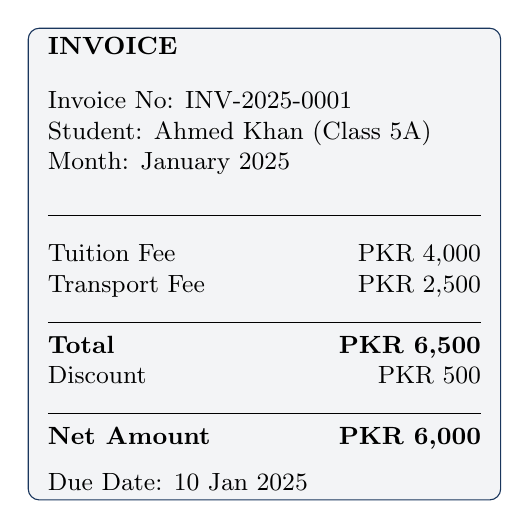
\begin{tikzpicture}[
    box/.style={draw=primaryblue, rounded corners, minimum width=6cm, 
                align=left, font=\small, fill=lightgray}
]
    \node[box, minimum height=5cm] at (0,0) {
        \textbf{INVOICE}\\[0.3cm]
        Invoice No: INV-2025-0001\\
        Student: Ahmed Khan (Class 5A)\\
        Month: January 2025\\[0.2cm]
        \rule{5.5cm}{0.4pt}\\[0.2cm]
        Tuition Fee \hfill PKR 4,000\\
        Transport Fee \hfill PKR 2,500\\
        \rule{5.5cm}{0.4pt}\\
        \textbf{Total} \hfill \textbf{PKR 6,500}\\
        Discount \hfill PKR 500\\
        \rule{5.5cm}{0.4pt}\\
        \textbf{Net Amount} \hfill \textbf{PKR 6,000}\\[0.2cm]
        Due Date: 10 Jan 2025
    };
\end{tikzpicture}
\end{center}

\section{Invoice Status}

\begin{longtable}{@{}p{3cm}p{4cm}p{5cm}@{}}
\toprule
\textbf{Status} & \textbf{Condition} & \textbf{Action} \\
\midrule
\endhead
Pending & No payment made & Awaiting payment \\
Partial & Paid $<$ Net Amount & Balance remaining \\
Paid & Paid = Net Amount & Complete \\
Overdue & Past due date + unpaid & Follow up needed \\
\bottomrule
\end{longtable}

% ============================================================================
% CHAPTER 5: PAYMENTS
% ============================================================================
\chapter{Payment Collection}

\section{Recording Payments}

Navigate to \texttt{Fees} $\rightarrow$ \texttt{Collect Payment}

\begin{enumerate}[leftmargin=*]
    \item Search and select student
    \item View pending invoices
    \item Select invoice(s) to pay
    \item Enter payment amount
    \item Select payment mode
    \item Enter reference details (if applicable)
    \item Confirm payment
    \item Print receipt
\end{enumerate}

\section{Payment Modes}

\begin{center}
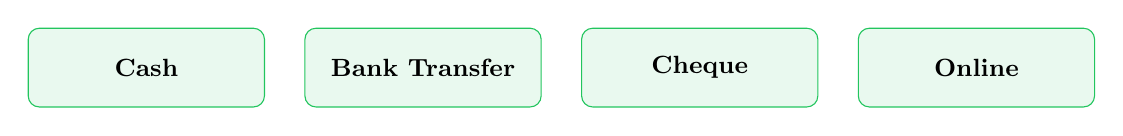
\begin{tikzpicture}[
    mode/.style={draw=accentgreen, rounded corners, minimum width=3cm, 
                 minimum height=1cm, fill=accentgreen!10, font=\small\bfseries}
]
    \node[mode] (cash) at (0,0) {Cash};
    \node[mode, right=0.5cm of cash] (bank) {Bank Transfer};
    \node[mode, right=0.5cm of bank] (cheque) {Cheque};
    \node[mode, right=0.5cm of cheque] (online) {Online};
\end{tikzpicture}
\end{center}

\subsection{Payment Mode Details}

\begin{longtable}{@{}p{3cm}p{10cm}@{}}
\toprule
\textbf{Mode} & \textbf{Required Information} \\
\midrule
\endhead
Cash & No additional details required \\
Bank Transfer & Bank name, Reference number \\
Cheque & Bank name, Cheque number, Cheque date \\
Online & Transaction ID, Platform name \\
\bottomrule
\end{longtable}

\section{Payment Receipt}

After successful payment:
\begin{itemize}[leftmargin=*]
    \item Receipt automatically generated
    \item Unique receipt number assigned
    \item Option to print or email receipt
    \item Invoice status updated automatically
\end{itemize}

% ============================================================================
% CHAPTER 6: CONCESSIONS
% ============================================================================
\chapter{Concessions \& Discounts}

\section{Overview}

Concessions allow you to apply discounts to student fees based on various criteria.

\section{Concession Types}

\begin{center}
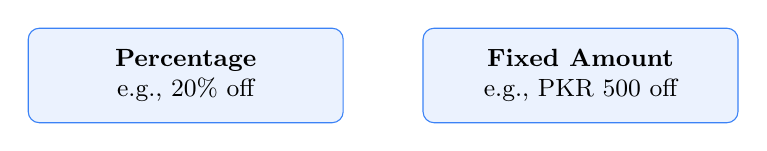
\begin{tikzpicture}[
    type/.style={draw=secondaryblue, rounded corners, minimum width=4cm, 
                 minimum height=1.2cm, fill=secondaryblue!10, align=center, 
                 font=\small}
]
    \node[type] (percent) at (0,0) {\textbf{Percentage}\\e.g., 20\% off};
    \node[type, right=1cm of percent] (fixed) {\textbf{Fixed Amount}\\e.g., PKR 500 off};
\end{tikzpicture}
\end{center}

\section{Creating Concessions}

Navigate to \texttt{Fees} $\rightarrow$ \texttt{Concessions} $\rightarrow$ \texttt{Add}

\begin{longtable}{@{}p{4cm}p{3cm}p{6cm}@{}}
\toprule
\textbf{Field} & \textbf{Required} & \textbf{Description} \\
\midrule
\endhead
Student & Yes & Select student \\
Fee Type & No & Specific fee or all fees \\
Discount Type & Yes & Percentage or Fixed \\
Discount Value & Yes & Amount or percentage \\
Reason & No & Reason for concession \\
Start Date & Yes & When concession begins \\
End Date & No & When concession ends \\
\bottomrule
\end{longtable}

\section{Common Concession Reasons}

\begin{itemize}[leftmargin=*]
    \item Sibling discount
    \item Staff child
    \item Merit scholarship
    \item Financial hardship
    \item Early payment discount
\end{itemize}

% ============================================================================
% CHAPTER 7: DEFAULTERS
% ============================================================================
\chapter{Defaulter Management}

\section{Identifying Defaulters}

Navigate to \texttt{Fees} $\rightarrow$ \texttt{Defaulters}

Defaulters are students with:
\begin{itemize}[leftmargin=*]
    \item Overdue invoices
    \item Balance exceeding threshold
    \item Multiple unpaid months
\end{itemize}

\section{Defaulter List}

\begin{center}
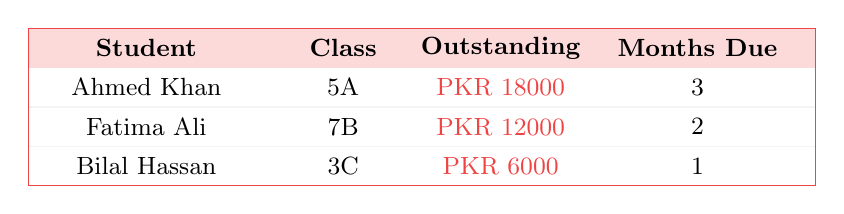
\begin{tikzpicture}
    % Header
    \fill[dangerred!20] (0,2) rectangle (10,2.5);
    \node[font=\small\bfseries] at (1.5,2.25) {Student};
    \node[font=\small\bfseries] at (4,2.25) {Class};
    \node[font=\small\bfseries] at (6,2.25) {Outstanding};
    \node[font=\small\bfseries] at (8.5,2.25) {Months Due};
    
    % Rows
    \foreach \y/\name/\class/\amount/\months in {
        1.5/Ahmed Khan/5A/18000/3,
        1/Fatima Ali/7B/12000/2,
        0.5/Bilal Hassan/3C/6000/1
    } {
        \draw[lightgray] (0,\y) -- (10,\y);
        \node[font=\small] at (1.5,\y+0.25) {\name};
        \node[font=\small] at (4,\y+0.25) {\class};
        \node[font=\small, text=dangerred] at (6,\y+0.25) {PKR \amount};
        \node[font=\small] at (8.5,\y+0.25) {\months};
    }
    
    \draw[dangerred] (0,0.5) rectangle (10,2.5);
\end{tikzpicture}
\end{center}

\section{Taking Action}

For each defaulter, you can:
\begin{itemize}[leftmargin=*]
    \item View complete fee history
    \item Send reminder notification
    \item Print outstanding statement
    \item Apply concession if needed
    \item Record partial payment
\end{itemize}

% ============================================================================
% CHAPTER 8: REPORTS
% ============================================================================
\chapter{Fee Reports}

\section{Available Reports}

\begin{longtable}{@{}p{4cm}p{9cm}@{}}
\toprule
\textbf{Report} & \textbf{Description} \\
\midrule
\endhead
Collection Report & Daily/monthly collections summary \\
Outstanding Report & All unpaid amounts \\
Defaulters Report & Students with overdue fees \\
Class-wise Report & Fee status by class \\
Invoice Report & All invoices with status \\
Payment Register & All payments with details \\
Concession Report & All discounts applied \\
\bottomrule
\end{longtable}

\section{Collection Summary}

\begin{center}

\begin{tikzpicture}[
    stat/.style={draw=primaryblue, rounded corners, minimum width=3.5cm, 
                 minimum height=2cm, fill=lightgray, align=center}
]
    \node[stat] (total) at (0,0) {
        \textbf{\large Total Billed}\\[0.2cm]
        \textcolor{primaryblue}{\LARGE PKR 1.2M}
    };
    \node[stat, right=0.5cm of total] (collected) {
        \textbf{\large Collected}\\[0.2cm]
        \textcolor{accentgreen}{\LARGE PKR 950K}
    };
    \node[stat, right=0.5cm of collected] (outstanding) {
        \textbf{\large Outstanding}\\[0.2cm]
        \textcolor{dangerred}{\LARGE PKR 250K}
    };
\end{tikzpicture}
\end{center}

\section{Exporting Reports}

\begin{enumerate}[leftmargin=*]
    \item Select report type
    \item Choose date range
    \item Apply filters (class, status)
    \item Select format (PDF / Excel)
    \item Click Export
\end{enumerate}

\end{document}
